\section{Auswertung}
\label{sec:auswertung}

\subsection{Eichung des Magnetfelds}
Um in den folgenden Auswertungsschritten
die jeweilige magnetische Flussdichte zu kennen,
wird zuerst eine Eichung des Elektromagneten durchgeführt,
wie in \autoref{sec:durchfuehrung} beschrieben.

Die entsprechenden Messwerte sind in \autoref{tab:eichung} angegeben
und in \autoref{fig:plt:eichung} grafisch dargestellt.

Mithilfe einer Regressionsrechnung unter Verwendung der Python-Bibliothek \texttt{numpy} % genauer: np.polyfit
ergeben sich folgende Parameter für ein Polynom dritten Grades
\[
    B(I) = aI^3 + bI^2 + cI + d
\]
mit den Parametern
\begin{align*}
    a &= \SI{-0.45 \pm 0.04}{\milli\tesla\per\cubic\ampere} \\
    b &= \SI{-0.1 \pm 0.4}{\milli\tesla\per\square\ampere} \\
    c &= \SI{100.7 \pm 1.5}{\milli\tesla\per\ampere} \\
    d &= \SI{1.1 \pm 1.4}{\milli\tesla} \ .
\end{align*}

\begin{table}
    \centering
    \caption{Magnetische Flussdichte in Abhängigkeit des Spulenstroms.}
    \label{tab:eichung}
    \begin{tabular}{S S}
        \toprule
        {$I \mathbin{/} \si{A}$} & {$B \mathbin{/} \si{\milli\tesla}$} \\
        \midrule
        0 & 0 \\
        0.5 & 100 \\
        \bottomrule
    \end{tabular}
\end{table}

\begin{figure}[H]
    \centering
    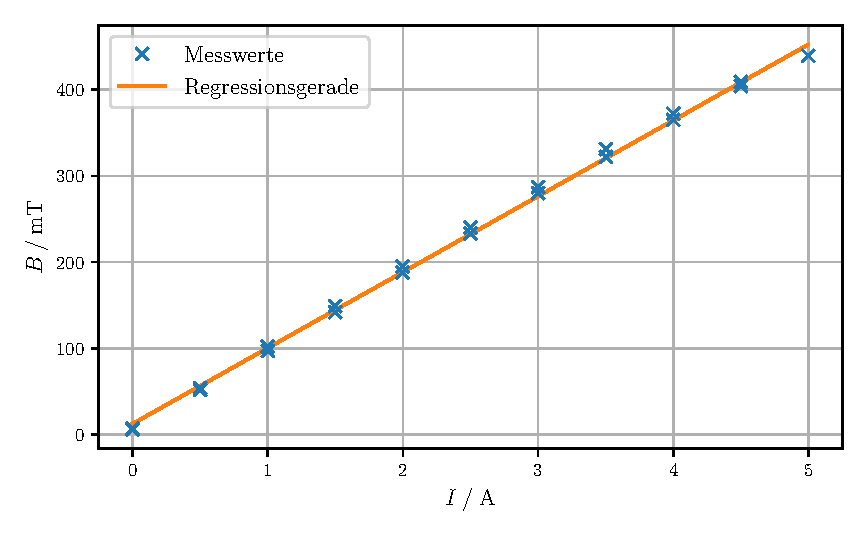
\includegraphics[width=\textwidth]{build/plt/1_magnet.pdf}
    \caption{Messwerte und Regressionspolynom zur Eichung des Elektromagneten.}
    \label{fig:plt:eichung}
\end{figure}

\subsection{Zur Umsetzung der Abstandsbestimmung von Spektrallinien}
Die Auswertung eines einzelnen Bilds erfolgt in den folgenden Schritten:
\begin{itemize}
    \item Die im Bild eingebettete Datumsangabe wird mit Schwarz übermalt, um die spätere Erkennung nicht zu stören.
    \item Das Bild wird so rotiert, dass die einzelnen Linien möglichst vertikal ausgerichtet sind.
    \item Da davon auszugehen ist, dass das Bild keine verwertbaren Farbinformationen enthält, werden die RGB-Kanäle summiert.
    \item Für jede Pixel-Spalte wird eine Summe gebildet, sodass ein eindimensionales Array verbleibt,
          welches auf den Wertebereich $[0, 1]$ normiert wird.
          % TODO: hyperlink, …
    \item Mittels \texttt{scipy.signal.TODO.find\_peaks} und gegebenenfalls angepasster Suchparameter (\texttt{prominence}, y, z)
          werden die Maxima ermittelt,
          welche den Linien entsprechen, deren Abstand bestimmt werden soll.
    \item Da die Abstände in beliebigen Einheiten verwendet werden können,
          muss nur noch die Differenz der Indizes (und somit der Pixel) je zweier Maxima berechnet werden.
    \item Aus den einzelnen Abständen wird schließlich das arithmetische Mittel gebildet.
\end{itemize}

\subsection{Untersuchung der roten Spektrallinie}
\lipsum[1]

\subsection{Untersuchung der blauen, sigma-polarisierten Spektrallinie}
\lipsum[1]

\subsection{Untersuchung der blauen, pi-polarisierten Spektrallinie}
\lipsum[1]
